\documentclass{standalone}
\begin{document}

    % MEDICAL DIGITAL IMAGES
    \documentclass{standalone}
\begin{document}
\chapter{Results}
This Chapter will be aimed to show and discuss the results of the developed pipeline.
First of all, a brief description of the Dataset provided by the IRCCS Sant’Orsola-Malpighi Policlinic will be provided.
Then, the accuracy of the segmentation and of the prediction of response.
Finally, the outputs of the implementation will be shown.

\end{document}

    % GENERAL PROPERTIES 
    \documentclass{standalone}
\begin{document}
\subsection{General Properties}
The physical meaning of the image data depends on the performed image modality.
For example, Computed Tomography (CT) and Magnetic Resonance Imaging (MRI), give structural information about the anatomy of the patient.
Other techniques, such as Positron Emission Tomography (PET) or Functional Magnetic Resonance Imaging (fMRI) give information about the functional properties of the patient's target organs. 
However, we can distinguish some general characteristics of digital images:

\paragraph{Pixel depth} is the number of bits used to encode the values of each pixel and it is related to the memory space used to store the amount of the encoded information\cite{Larobina}. 
Higher the number of bits, higher the information stored but more memory space is required\cite{Larobina}. 
A group of 8 bits is called \textit{byte} and represent the smallest quantity that can be stored in the memory of a computer.
For example, if an image has a pixel depth of 16 or 12 bits the computer will always store two bytes per pixel\cite{Larobina}.
With a pixel depth of 8 bits it is possible to codify and store integer numbers between 0 and 255 $(2^8-1)$.
There are also two formats for the encoding in binary of floating-point numbers: single precision 32-bit and double precision 64-bit.

\paragraph{Pixel data} represent numerical values of the pixels stored according to the data type.
Pixel data can be complex values even if this data type is not common and can be bypassed by storing the real and imaginary parts as separate images.
For example, complex data are provided in MRI acquired data before the reconstruction (the so called k-space)\cite{Larobina}.


\paragraph{Metadata} are information that describe the image. It is usually stored at the beginning of the file as a header\cite{Larobina}. 
In the case of medical images, metadata have an important role due to the nature of the images.
For example, a magnetic resonance image might have parameters related to the pulse sequence used, timing information, number of acquisitions while a PET image might have information about the radiopharmaceutical injected and the weight of the patient.


\end{document}

        % MEDICAL IMAGE FORMATS
        \documentclass{standalone}
\begin{document}
    
\subsubsection{DICOM Format}

Image file formats provide a standard way to store information of an image in a computer file\cite{biondi}.
DICOM is the acronym of Digital Imaging and COmmunications in medicine.
It is not only a file format but also a network communication protocol\cite{Larobina}.
However here, we will discuss DICOM only as a medical image format.\\
DICOM file format establishes that the pixel data cannot be separated from the metadata\cite{Larobina}.
In other words, metadata and pixel data are merged in a unique file.
The header contains the description of the entire procedure used to generate the image in terms of acquisition protocol and scanning parameters\cite{Larobina}. 
It also contains patient information such as name, gender, age. 
For these reasons, the DICOM header is modality-dependent and varies in size. 
In practice, the header allows the image to be \textit{self-descriptive}.

\end{document}

    \newpage
    % SPATIAL DOMAIN FILTERING
    \documentclass{standalone}
\begin{document}
\section{Spatial Domain Filtering}


Filtering is a procedure used for modifying or enhancing an image.
The value of any given pixel in the output image is determined by applying some operations to the neighborhood of the corresponding input pixel.
A pixel's neighborhood is some set of pixels, defined by their locations relative to that pixel.
The term \textit{spatial domain} indicates that the procedures operate directly on pixels.
Mathematically:

\begin{equation}
    g(x,y) = T[f(x,y)] 
\end{equation}

where $f(x, y)$ is the input image, $g(x, y)$ the output image and $T$ is an operator on $f$ defined over some neighborhood of $(x, y)$.
The operation on the point located in $(x, y)$ usually involves the application of a matrix called \textit{mask} or \textit{kernel}.
The application of the above-mentioned mask (or kernel) on an image is called \textit{spatial filtering}.
Filtering creates a new pixel with the same coordinates of the center of the neighborhood, whose value is the result of the operation.
For each $(x, y)$ of the image, the filter transform $g(x, y)$ is the linear combination of the mask coefficient $w(s, t)$ and the pixels of the image affected by the mask itself.
In general, we can write:
\begin{equation}
    g(x, y) = \sum_{s = -a}^{a} \sum_{t = -b}^{b} w(s, t) f(x + s, y + t)
\end{equation}  

\begin{figure}[ht]

    \centering
    \includegraphics[width=.9\textwidth]{../images/filtering.png}
    
    \caption{Example of spatial filtering. A filtered image is generated as the center of the mask or kernel, moves to every pixel in the input image. From \cite{filtering}}
    \label{filtering}
\end{figure}


\end{document}

        % SPATIAL FILTER
        \documentclass{standalone}
\begin{document}
\subsection{Spatial Filter}

A spatial filter consists in a (usually square) region called \textit{mask}  and a pre-defined operation applied on pixels of the region covered by the mask\cite{corrandconv}.
Filtering creates a new pixel with the same coordinates as the center of the neighborhood whose value is the result of the operation.
For each $(x, y)$ of the image, the filter transform $g(x, y)$ is the linear combination of the mask coefficient $w(s, t)$ and the pixels of the image affected by the mask itself.
\\
In general, we can write:
\begin{equation}
    g(x, y) = \sum_{s = -a}^{a} \sum_{t = -b}^{b} w(s, t) f(x + s, y + t)
\end{equation}  


\end{document}

        % CORRELATION AND CONVOLUTION
        \documentclass{standalone}
\begin{document}
\subsection{Correlation and Convolution}


Spatial filtering is a correlation or convolution process.
Correlation is the process of moving a \textit{mask} or \textit{kernel} over the image and computing the sum of products at each location\cite{corrandconv}.
The mechanics of convolution are the same, except that the filter is first rotated by $180^{\circ}$ degree.
In other words, correlation or convolution are filter shift functions.\\
The correlation and convolution of a filter $w(x, y$) of size $m \times n$ with an image $f(x, y)$ can be written as follow:

\begin{align}
    Correlation:  w(s, t) \times f(x, y) = & \sum_{s = -a}^{a} \sum_{t = -b}^{b} w(s, t) f(x + s, y + t) \\
    Convolution:  w(s, t) \circledast f(x, y) = & \sum_{s = -a}^{a} \sum_{t = -b}^{b} w(s, t) f(x - s, y - t) 
\end{align}


\end{document}

        % SMOOTHING FILTERS
        \documentclass{standalone}
\begin{document}
\subsection{Smoothing Filters}
Smoothing filters are used for blurring and for noise reduction\cite{corrandconv}.
This is used in removal of small details and bridging of small gaps in lines or curves.
Smoothing spatial filters include \textit{linear filters} and \textit{nonlinear filters}\cite{corrandconv}.\\
The general implementation for filtering an $M \times N$ image with a weighted averaging filter of size $m \times n$ is given by:
\begin{equation}
    g(x, y) = \frac{\sum_{s = -a}^{a} \sum_{t = -b}^{b} w(s, t) f(x + s, y + t)}{\sum_{s = -a}^{a} \sum_{t = -b}^{b} w(s, t)}
\end{equation}
where $m=2a+1$ and $n=2b+1$.

\paragraph{Linear filtering} is based on the \textit{mean filter} \cite{filters}.
The mean filter is a simple sliding spatial filter that replaces the center value in the mask region with the average of all the neighboring pixel values including itself. 
These filters are also called \textit{low pass filters} since the process of averaging drastically lowers high frequencies.
The mask or kernel is a square.
Larger kernels ($5\times5$ or $7\times7$) produce more denoising that smaller ones ($3 \times 3$) but make the image more blurred\cite{filters}. 
A common mean filter can be described by a $3\times3$ matrix with all elements equal to 1, so that the output pixel corresponds to a value of:

\begin{equation}
    R = \frac{1}{9} \begin{pmatrix}
        1 & 1 & 1\\
        1 & 1 & 1\\
        1 & 1 & 1
        \end{pmatrix} \mathbf{z} = \frac{1}{9} \sum_{i = 1}^{9}z_i
\end{equation}

 or using a weighted mean filter:

\begin{equation}
     R' = \frac{1}{16}\begin{pmatrix}
        1 & 2 & 1\\
        2 & 4 & 2\\
        1 & 2 & 1
        \end{pmatrix} \mathbf{z}
\end{equation}






\paragraph{Non-Linear filtering} is based on the \textit{median filter}\cite{filters}.
The median filter principle is similar to the mean filter. 
The mask or kernel is scanned over the pixels of the entire image.
The median of the pixel values in the mask region is calculated, and the center pixel of the mask region is replaced with the calculated median value\cite{filters}.
This filter is particularly effective in the presence of \textit{impulse noise} (or \textit{salt-and-pepper noise})\cite{corrandconv}.\\
Mathematically:

\begin{equation}
    g(p) = median\{f(p), where \: p \in N_8(p)\}
\end{equation}
where $g(p)$ is the median pixel value, $f(p)$ all pixel values under mask, and $N_8(p)$ 8-neighborhood of pixel $p$.


\paragraph{\textcolor{blue}{Notes:} Adaptive filters} 
are commonly used in image processing to enhance or restore data by removing noise without significantly blurring the structures in the image\cite{Adaptive}.
This means not smoothing the areas of the image in which there is a large jump in intensity values (i.e. when there is an \textit{edge}) and at the same time applying the filter to lower the noise.
In this case, the local variance will be evaluated concerning the variance of the noise that occurs.\\
Mathematically:
\begin{equation}
    \hat{f}(x, y) = f(x, y) - \frac{\sigma_{noise}^2}{\sigma_{local}^2}[f(x, y) - m_{local}]
\end{equation}

\end{document}


    \newpage
    % SEGMENTATION
    \documentclass{standalone}
\usepackage{xr}
\externaldocument{../Chapter2/intro}
\begin{document}
\subsection{Segmentation}
Once trained, the CNN model was used for the segmentation of the MRI scans of each patient.
Before the segmentation, the scans are pre-processed as previously described.
\\
The segmentation is done slice by slice, for each patient, by using the trained CNN model to obtain the predicted tumor area.
The prediction values range between 0 and 1.
\\
Then, using \textsc{OpenCV}\cite{opencv_library} functions it is possible to obtain a segmented area like the one in Figure \ref{contoured}, where the red contour represents the border of the predicted tumor area.


\begin{figure}[htp]

    \centering
    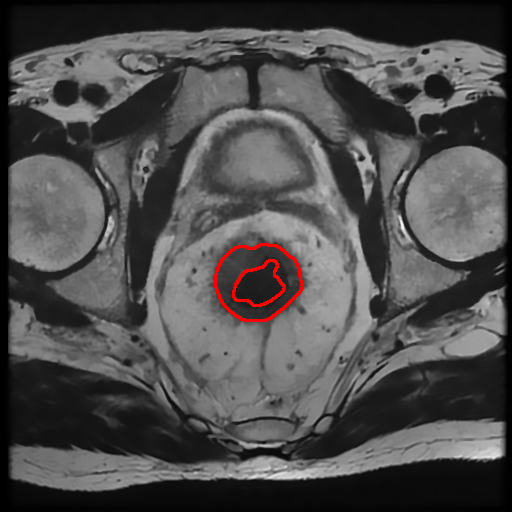
\includegraphics[width=.49\textwidth]{../images/BO56_9_cont.png}
    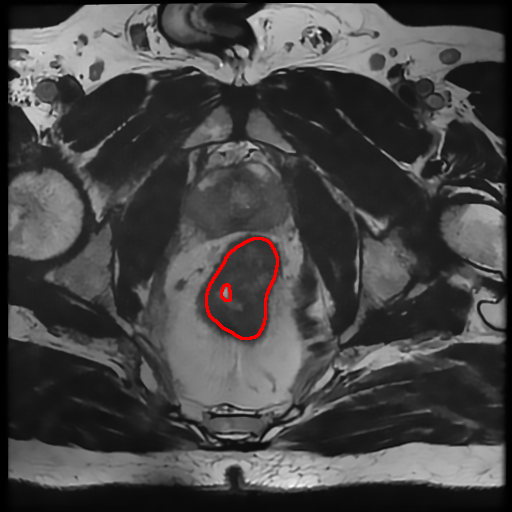
\includegraphics[width=.49\textwidth]{../images/BO85_6_cont.png}
    
    \caption{Images of colorectal cancer with identified tumor areas from two different patients. The red contour represents the border of the predicted tumor area.}
    \label{contoured}
    
    \end{figure}


\end{document}
        % METHODS
        \documentclass{standalone}
\begin{document}
\subsection{Methods}
During the year several segmentation methods have been developed\cite{biondi}.
There are several ways to classify these methods.
For example, depending if they require or not a training set of data, they can be classified into \textit{supervised} or \textit{unsupervised} methods.
More, they can be classified depending on the information type they use, like \textit{Pixel classification} methods, which use only information about pixel intensity, or \textit{Boundary following} methods which use edge information etc...\cite{biondi}.\\
Among the most common ones:

\paragraph{Thresholding}
is a very simple and common approach to segmentation.
This method is applied on the \textit{histogram} of the image.
The histogram of a digital image with intensity levels $L$ in the range $[0, \: L-1]$, is a discrete function $h(l_k) = n_k$ where $l_k$ is the k-th intensity value and $n_k$  is the number of pixels with intensity $l_k$.\\
Thresholding consists in binarizing an image through an (if) clause on the intensity value of each point after having determined a threshold value $T \in [0, \: L-1]$.
The threshold value $T$ is usually chosen by visual assessment on the image histogram but it can be automatize by algorithms like the \textit{Otsu algorithm}.
One drawback of this method is that some parts of the image can belong to the same class even if they belong to different objects.
In fact, thresholding does not take into account the spatial characteristics of the image.
Moreover, it is sensitive to noise and intensity inhomogeneity that corrupt the image histogram and make difficult the classification of pixels\cite{biondi}.

\begin{figure}[htp]

    \centering
    \includegraphics[width=.45\textwidth]{../images/thresholdhistogram.png}
    \includegraphics[width=.45\textwidth]{../images/thresholdexample.png}
    
    \caption{Example of thresholding segmentation using Fiji software\cite{Fiji}. \\
    \textit{ Left)} Image Histogram.\textit{ Right)} Result of thresholding.}
    \label{thresholding}
    
    \end{figure}


\paragraph{Artificial Neural Networks} 
are computational architectures derived from neural physiological models\cite{segmentationreview}.
Artificial Neural Networks (ANNs) have evolved into a broad family of techniques.
For visual analysis are usually used Convolutional Neural Networks (CNNs) based on \textit{convolution kernels} or \textit{filters} that slide along input data to extract feature maps\cite{wiki:cnn}.
Several architectures have been developed over the years, for different tasks and fields of application.
In bio-medical image processing, the so-called U-Net\cite{unet}, is one of the most common architecture.
U-Net is a kind of CNN which allows overcoming the requirement of many training data\cite{biondi, unet}.
However a better explanation of ANNs will be provided in the following chapter.




\end{document}

    \newpage
    % RADIOMICS
    \documentclass{standalone}
\begin{document}
\section{Radiomics}
Radiomics consists in methods that extract from medical images a large number of features, which have the potential to uncover disease characteristics that fail to be appreciated by the naked eye\cite{wiki:Radiomics}.
The main objective of radiomics is to assist the subjective interpretation of the clinicians with an objective prediction.
In the new era of precision medicine, radiomics is an emerging translational research field that aims to find associations between qualitative and quantitative information extracted from clinical images and clinical data to support the decision making process\cite{tesicoppola}.
Radiomic features can be divided into different classes:
\begin{itemize}
    \item First Order Statistics
    \item Shape based features 2D and 3D
    \item Gray Level Co-occurrence Matrix (GLCM)
    \item Gray Level Size Zone (GLSZM)
    \item Gray Level Run Length Matrix (GLRLM)
    \item Neighbouring Gray Tone Difference Matrix (NGTDM)
    \item Gray Level Dependence Matrix (GLDM)
\end{itemize}

\end{document}

        % RADIOMIC FEATURES
        \documentclass{standalone}
\begin{document}
\subsection{Radiomic Features}

Radiomic features can be divided into five groups\cite{wiki:Radiomics, tesicoppola}:
\begin{itemize}
    \item size and shape based–features like descriptors of the image intensity histogram, gray-level co-occurrence matrix (GLCM);
    \item run length matrix (RLM);
    \item size zone matrix (SZM);
    \item neighborhood gray tone difference matrix (NGTDM) derived textures, textures extracted from filtered images;
    \item fractal features.
\end{itemize}
\end{document}

        % POSSIBLE PURPOSES OF RADIOMICS
        \documentclass{standalone}
\begin{document}
\subsection{Possible Purposes Of Radiomics}

The possible applications of radiomics are based on a very wide range, from the prediction of clinical outcomes to the oncological diagnosis.
In this subsection, a brief overview of some general possible purposes will be given.
\subsubsection{Prediction of clinical outcomes} 
Radiomic features may be useful for predicting patient survival and describing intratumoral heterogeneity as demonstrated in a study by Aerts et al. \cite{Aerts}.
More, the usefulness of radiomics for predicting the immunotherapy response of patients with non-small cell lung cancer (NSCLC) using pretreatment CT and PET-CT images has been demonstrated by other studies\cite{tesicoppola}.
\subsubsection{Prediction of metastases}
Radiomic features can also predict the metastatic stage of tumors. 
For example, many radiomic features were identified as predictors of distant metastasis of lung adenocarcinoma in a study by Coroller et al.\cite{Coroller}.
They concluded that radiomic features may be useful in identifying patients at high risk of developing distant metastases, guiding clinicians in choosing the most effective treatment for individual patients.
\subsubsection{Prediction of physiological events}
Another possible application of radiomics analysis is the prediction of physiological events. 
Indeed, radiomics can be applied for the characterization and investigation of complex physiological events such as brain activity, which is usually studied with specific imaging techniques such as functional magnetic resonance ”fMRI”\cite{tesicoppola}. 


\end{document}

\end{document}